\chapter[Data about the languages featured in the problems]{Data about the languages featured in the problems: Family, number of native speakers, region}
\label{appendix:1}

% \noindent
% \begin{longtable}{|l|m{5.8em}|m{6em}|m{3.5em}|m{8em}|}
% \hline
% \rotatebox[origin=c]{90}{Prob. No.} & {Language} & {Family}\footnote{IE = \famIndoEuropean, TNG = \famTNG.} & {NS}\footnote{Native speakers. bil. = billion, mil. = million, ? = unknown.} & {Region} \\ \hline
\begin{description}[font=\normalfont,style=nextline]\multicolsep=0pt\columnsep=-1em
\item[\langnameAcehnese] 
 \begin{multicols}{2}\begin{description}[font=\normalfont\itshape,noitemsep] 
 \item[]
 \item[\pbnumberabbr] 5.8 
 \item[\family] \famAustronesian 
 \item[]
\item[\nativespeakers] 3.37 mil. 
 \item[\region] \regionIndonesia 
 \end{description}\end{multicols}
\item[\langnameAfrihili] 
 \begin{multicols}{2}\begin{description}[font=\normalfont\itshape,noitemsep] 
 \item[] 
 \item[\pbnumberabbr] 5.12 
 \item[\family] \famConstructed 
 \item[]
\item[\nativespeakers] 0 
 \item[\region] --
 \end{description}\end{multicols}
\item[\langnameAinu] 
 \begin{multicols}{2}\begin{description}[font=\normalfont\itshape,noitemsep] 
 \item[] 
 \item[\pbnumberabbr] 6.13 
 \item[\family] \famIsolated 
 \item[]
\item[\nativespeakers] 2 
 \item[\region] \regionHokkaido\ \Brackets{\regionJapan} 
 \end{description}\end{multicols}
\item[\langnameAkan] 
 \begin{multicols}{2}\begin{description}[font=\normalfont\itshape,noitemsep] 
 \item[] 
 \item[\pbnumberabbr] 10.9 
 \item[\family] \famNigerCongo 
 \item[]
\item[\nativespeakers] 11 mil. 
 \item[\region] \regionGhana\EnumComma\regionIvoryCoast\EnumComma\regionTogo 
 \end{description}\end{multicols}
\item[\langnameAlabama] 
 \begin{multicols}{2}\begin{description}[font=\normalfont\itshape,noitemsep] 
 \item[] 
 \item[\pbnumberabbr] 5.8  
 \item[\family] \famMuskogean 
 \item[]
\item[\nativespeakers] 370 
 \item[\region] \regionTexas\ \Brackets{\regionUSA}
 \end{description}\end{multicols}
\item[\langnameAlamblak] 
 \begin{multicols}{2}\begin{description}[font=\normalfont\itshape,noitemsep] 
 \item[] 
 \item[\pbnumberabbr] 9.14 
 \item[\family] \famSepik 
 \item[]
\item[\nativespeakers] 1,500 
 \item[\region] \regionPNG 
 \end{description}\end{multicols}
\item[\langnameArabic] 
 \begin{multicols}{2}\begin{description}[font=\normalfont\itshape,noitemsep] 
 \item[] 
 \item[\pbnumberabbr] 2.9\EnumComma4.9\EnumComma7.7 
 \item[\family] \famAfroasiatic 
 \item[]
\item[\nativespeakers] 350 mil. 
 \item[\region] \regionAsia\EnumComma\regionAfrica 
 \end{description}\end{multicols}

\pagebreak
\item[\langnameAralle] 
 \begin{multicols}{2}\begin{description}[font=\normalfont\itshape,noitemsep] 
 \item[] 
 \item[\pbnumberabbr] 10.8 
 \item[\family] \famAustronesian 
 \item[]
\item[\nativespeakers] 12,000 
 \item[\region] \regionWSulawesi\ \Brackets{\regionIndonesia} 
 \end{description}\end{multicols}
\item[\langnameArawak] 
 \begin{multicols}{2}\begin{description}[font=\normalfont\itshape,noitemsep] 
 \item[] 
 \item[\pbnumberabbr] 10.2 
 \item[\family] \famArawakan 
 \item[]
\item[\nativespeakers] 2,510 
 \item[\region] \regionSouthAmerica 
 \end{description}\end{multicols}
\item[\langnameArmenian] 
 \begin{multicols}{2}\begin{description}[font=\normalfont\itshape,noitemsep] 
 \item[] 
 \item[\pbnumberabbr] 2.5 
 \item[\family] \famIndoEuropean 
 \item[]
\item[\nativespeakers] 6.7 mil. 
 \item[\region] \regionArmenia 
 \end{description}\end{multicols}
\item[\langnameBardi] 
 \begin{multicols}{2}\begin{description}[font=\normalfont\itshape,noitemsep] 
 \item[] 
 \item[\pbnumberabbr] 10.3 
 \item[\family] \famNyulnyulan 
 \item[]
\item[\nativespeakers] 4 
 \item[\region] \regionAustralia 
 \end{description}\end{multicols}
\item[\langnameBari] 
 \begin{multicols}{2}\begin{description}[font=\normalfont\itshape,noitemsep] 
 \item[] 
 \item[\pbnumberabbr] 4.13\EnumComma5.8 
 \item[\family] \famNiloSaharan 
 \item[]
\item[\nativespeakers] 750,000 
 \item[\region] \regionSSudan 
 \end{description}\end{multicols}
\item[\langnameBasque] 
 \begin{multicols}{2}\begin{description}[font=\normalfont\itshape,noitemsep] 
 \item[] 
 \item[\pbnumberabbr] 8.3 
 \item[\family] \famIsolated 
 \item[]
\item[\nativespeakers] 750,000 
 \item[\region] \regionFrance\EnumComma\regionSpain 
 \end{description}\end{multicols}
\item[\langnameBeja] 
 \begin{multicols}{2}\begin{description}[font=\normalfont\itshape,noitemsep] 
 \item[] 
 \item[\pbnumberabbr] 7.4 
 \item[\family] \famAfroasiatic 
 \item[]
\item[\nativespeakers] 1-2 mil. 
 \item[\region] \regionSudan\EnumComma\regionEritrea\EnumComma\regionEgypt 
 \end{description}\end{multicols}
\item[\langnameBulgarian] 
 \begin{multicols}{2}\begin{description}[font=\normalfont\itshape,noitemsep] 
 \item[] 
 \item[\pbnumberabbr] 5.4 
 \item[\family] \famIndoEuropean 
 \item[]
\item[\nativespeakers] 8 mil. 
 \item[\region] \regionBulgaria 
 \end{description}\end{multicols}
\item[\langnameBurushaski] 
 \begin{multicols}{2}\begin{description}[font=\normalfont\itshape,noitemsep] 
 \item[] 
 \item[\pbnumberabbr] 7.11 
 \item[\family] \famIsolated 
 \item[]
\item[\nativespeakers] 112,000 
 \item[\region] \regionPakistan 
 \end{description}\end{multicols}
\item[\langnameChabu] 
 \begin{multicols}{2}\begin{description}[font=\normalfont\itshape,noitemsep] 
 \item[] 
 \item[\pbnumberabbr] 9.15 
 \item[\family] \famIsolated 
 \item[]
\item[\nativespeakers] 400 
 \item[\region] \regionEthiopia 
 \end{description}\end{multicols}
\item[\langnameChickasaw] 
 \begin{multicols}{2}\begin{description}[font=\normalfont\itshape,noitemsep] 
 \item[] 
 \item[\pbnumberabbr] 3.8 
 \item[\family] \famMuskogean 
 \item[]
\item[\nativespeakers] 75 
 \item[\region] \regionSOklahoma\ \Brackets{\regionUSA}
 \end{description}\end{multicols}

\pagebreak
\item[\langnameChinese] 
 \begin{multicols}{2}\begin{description}[font=\normalfont\itshape,noitemsep] 
 \item[] 
 \item[\pbnumberabbr] 8.5 
 \item[\family] \famSinoTibetan 
 \item[]
\item[\nativespeakers] 1.2 bil. 
 \item[\region] \regionChina 
 \end{description}\end{multicols}
\item[\langnameChuvash] 
 \begin{multicols}{2}\begin{description}[font=\normalfont\itshape,noitemsep] 
 \item[] 
 \item[\pbnumberabbr] 3.4 
 \item[\family] \famTurkic 
 \item[]
\item[\nativespeakers] 1 mil. 
 \item[\region] \regionRussia 
 \end{description}\end{multicols}
\item[\langnameCree] 
 \begin{multicols}{2}\begin{description}[font=\normalfont\itshape,noitemsep] 
 \item[] 
 \item[\pbnumberabbr] 6.12 
 \item[\family] \famAlgic 
 \item[]
\item[\nativespeakers] 96,000 
 \item[\region] \regionCanada\EnumComma\regionUSA 
 \end{description}\end{multicols}
\item[\langnameTicuna] 
 \begin{multicols}{2}\begin{description}[font=\normalfont\itshape,noitemsep] 
 \item[] 
 \item[\pbnumberabbr] 4.14 
 \item[\family] \famIsolated 
 \item[]
\item[\nativespeakers] 63,000 
 \item[\region] \regionBrazil\EnumComma\regionColumbia\EnumComma\regionPeru 
 \end{description}\end{multicols}
\item[\langnameCzech] 
 \begin{multicols}{2}\begin{description}[font=\normalfont\itshape,noitemsep] 
 \item[] 
 \item[\pbnumberabbr] 9.7 
 \item[\family] \famIndoEuropean 
 \item[]
\item[\nativespeakers] 14 mil. 
 \item[\region] \regionCzechia 
 \end{description}\end{multicols}
\item[\langnameDabida] 
 \begin{multicols}{2}\begin{description}[font=\normalfont\itshape,noitemsep] 
 \item[] 
 \item[\pbnumberabbr] 6.2 
 \item[\family] \famNigerCongo 
 \item[]
\item[\nativespeakers] 370,000 
 \item[\region] \regionKenya 
 \end{description}\end{multicols}
\item[\langnameDanish] 
 \begin{multicols}{2}\begin{description}[font=\normalfont\itshape,noitemsep] 
 \item[] 
 \item[\pbnumberabbr] 9.9 
 \item[\family] \famIndoEuropean 
 \item[]
\item[\nativespeakers] 6 mil. 
 \item[\region] \regionDenmark 
 \end{description}\end{multicols}
\item[\langnameDaza] 
 \begin{multicols}{2}\begin{description}[font=\normalfont\itshape,noitemsep] 
 \item[] 
 \item[\pbnumberabbr] 5.8 
 \item[\family] \famNiloSaharan 
 \item[]
\item[\nativespeakers] 380,000 
 \item[\region] \regionChad\EnumComma\regionNiger\EnumComma\regionSudan\EnumComma\regionLibya 
 \end{description}\end{multicols}
\item[\langnameDinka] 
 \begin{multicols}{2}\begin{description}[font=\normalfont\itshape,noitemsep] 
 \item[] 
 \item[\pbnumberabbr] 6.15 
 \item[\family] \famNiloSaharan 
 \item[]
\item[\nativespeakers] 1.3 mil. 
 \item[\region] \regionSudan 
 \end{description}\end{multicols}
\item[\langnameDutch] 
 \begin{multicols}{2}\begin{description}[font=\normalfont\itshape,noitemsep] 
 \item[] 
 \item[\pbnumberabbr] 4.11 
 \item[\family] \famIndoEuropean 
 \item[]
\item[\nativespeakers] 25 mil. 
 \item[\region] \regionNetherlands 
 \end{description}\end{multicols}
\item[\langnameDyirbal] 
 \begin{multicols}{2}\begin{description}[font=\normalfont\itshape,noitemsep] 
 \item[] 
 \item[\pbnumberabbr] 7.2 
 \item[\family] \famPamaNyungan 
 \item[]
 \item[]
\item[\nativespeakers] 8 
 \item[\region] \regionNEQueensland\ \Brackets{\regionAustralia}
 \end{description}\end{multicols}
\item[\langnameEmbaloh] 
 \begin{multicols}{2}\begin{description}[font=\normalfont\itshape,noitemsep] 
 \item[] 
 \item[\pbnumberabbr] 10.5 
 \item[\family] \famAustronesian 
 \item[]
\item[\nativespeakers] 10,000 
 \item[\region] \regionIndonesia 
 \end{description}\end{multicols}
\item[\langnameChami] 
 \begin{multicols}{2}\begin{description}[font=\normalfont\itshape,noitemsep] 
 \item[] 
 \item[\pbnumberabbr] 9.2 
 \item[\family] \famChocoan 
 \item[]
\item[\nativespeakers] 7,800 
 \item[\region] \regionColumbia 
 \end{description}\end{multicols}
\item[\langnameEnglish] 
 \begin{multicols}{2}\begin{description}[font=\normalfont\itshape,noitemsep] 
 \item[] 
 \item[\pbnumberabbr] 2.7 
 \item[\family] \famIndoEuropean 
 \item[]
 \item[]
\item[\nativespeakers] 1.2 bil. 
 \item[\region] \regionUK\EnumComma\regionUSA\EnumComma\regionAustralia\EnumComma\regionNewZealand 
 \end{description}\end{multicols}
\item[\langnameEstonian] 
 \begin{multicols}{2}\begin{description}[font=\normalfont\itshape,noitemsep] 
 \item[] 
 \item[\pbnumberabbr] 4.12\EnumComma9.10 
 \item[\family] \famUralic 
 \item[]
\item[\nativespeakers] 1.1 mil. 
 \item[\region] \regionEstonia 
 \end{description}\end{multicols}
\item[\langnameEvenki] 
 \begin{multicols}{2}\begin{description}[font=\normalfont\itshape,noitemsep] 
 \item[] 
 \item[\pbnumberabbr] 4.5 
 \item[\family] \famTungusic 
 \item[]
\item[\nativespeakers] 26,580 
 \item[\region] \regionChina\EnumComma\regionRussia 
 \end{description}\end{multicols}
\item[\langnameFijian] 
 \begin{multicols}{2}\begin{description}[font=\normalfont\itshape,noitemsep] 
 \item[] 
 \item[\pbnumberabbr] 3.6\EnumComma5.6 
 \item[\family] \famAustronesian 
 \item[]
\item[\nativespeakers] 340,000 
 \item[\region] \regionFiji 
 \end{description}\end{multicols}
\item[\langnameFinnish] 
 \begin{multicols}{2}\begin{description}[font=\normalfont\itshape,noitemsep] 
 \item[] 
 \item[\pbnumberabbr] 4.12 
 \item[\family] \famUralic 
 \item[]
\item[\nativespeakers] 5.8 mil. 
 \item[\region] \regionFinland 
 \end{description}\end{multicols}
\item[\langnameFitzroy] 
 \begin{multicols}{2}\begin{description}[font=\normalfont\itshape,noitemsep] 
 \item[] 
 \item[\pbnumberabbr] 5.8 
 \item[\family] \famPamaNyungan 
 \item[]
\item[\nativespeakers] Unknown 
 \item[\region] \regionQueensland\ \Brackets{\regionAustralia} 
 \end{description}\end{multicols}
\item[\langnameGee] 
 \begin{multicols}{2}\begin{description}[font=\normalfont\itshape,noitemsep] 
 \item[] 
 \item[\pbnumberabbr] 6.9 
 \item[\family] \famNigerCongo 
 \item[]
\item[\nativespeakers] 330,000 
 \item[\region] \regionTogo\EnumComma\regionBenin 
 \end{description}\end{multicols}
\item[\langnameGeez] 
 \begin{multicols}{2}\begin{description}[font=\normalfont\itshape,noitemsep] 
 \item[] 
 \item[\pbnumberabbr] 6.3 
 \item[\family] \famAfroasiatic 
 \item[]
\item[\nativespeakers] Extinct 
 \item[\region] \regionEritrea\EnumComma\regionEthiopia 
 \end{description}\end{multicols}
\item[\langnameGreek] 
 \begin{multicols}{2}\begin{description}[font=\normalfont\itshape,noitemsep] 
 \item[] 
 \item[\pbnumberabbr] 3.5\EnumComma5.7 
 \item[\family] \famIndoEuropean 
 \item[]
\item[\nativespeakers] 13.5 mil. 
 \item[\region] \regionGreece 
 \end{description}\end{multicols}
\item[\langnameGuarani] 
 \begin{multicols}{2}\begin{description}[font=\normalfont\itshape,noitemsep] 
 \item[] 
 \item[\pbnumberabbr] 8.2 
 \item[\family] \famTupian 
 \item[]
 \item[]
 \item[\nativespeakers] 6.5 mil. 
 \item[\region] \regionParaguay\EnumComma\regionBolivia\EnumComma\regionArgentina\EnumComma\regionBrazil 
 \end{description}\end{multicols}
\item[\langnameGyarung] 
 \begin{multicols}{2}\begin{description}[font=\normalfont\itshape,noitemsep] 
 \item[] 
 \item[\pbnumberabbr] 6.10 
 \item[\family] \famSinoTibetan 
 \item[]
\item[\nativespeakers] 83,000 
 \item[\region] \regionSichuan\ \Brackets{\regionChina}
 \end{description}\end{multicols}
\item[\langnameHakhun] 
 \begin{multicols}{2}\begin{description}[font=\normalfont\itshape,noitemsep] 
 \item[] 
 \item[\pbnumberabbr] 6.11 
 \item[\family] \famSinoTibetan 
 \item[]
\item[\nativespeakers] 108,000 
 \item[\region] \regionBurma\EnumComma\regionIndia 
 \end{description}\end{multicols}
\item[\langnameHanunoo] 
 \begin{multicols}{2}\begin{description}[font=\normalfont\itshape,noitemsep] 
 \item[] 
 \item[\pbnumberabbr] 5.8 
 \item[\family] \famAustronesian 
 \item[]
\item[\nativespeakers] 13,000 
 \item[\region] \regionPhilippines 
 \end{description}\end{multicols}
\item[\langnameHausa] 
 \begin{multicols}{2}\begin{description}[font=\normalfont\itshape,noitemsep] 
 \item[] 
 \item[\pbnumberabbr] 5.8\EnumComma8.6 
 \item[\family] \famAfroasiatic 
 \item[]
 \item[]
\item[\nativespeakers] 60 mil. 
 \item[\region] \regionNigeria\EnumComma\regionNiger\EnumComma\regionCameroon\EnumComma\regionBenin\EnumComma\regionChad 
 \end{description}\end{multicols}
\item[\langnameHebrew] 
 \begin{multicols}{2}\begin{description}[font=\normalfont\itshape,noitemsep] 
 \item[] 
 \item[\pbnumberabbr] 2.9 
 \item[\family] \famAfroasiatic 
 \item[]
\item[\nativespeakers] 9 mil. 
 \item[\region] \regionIsrael 
 \end{description}\end{multicols}
\item[\langnameHmong] 
 \begin{multicols}{2}\begin{description}[font=\normalfont\itshape,noitemsep] 
 \item[] 
 \item[\pbnumberabbr] 2.1 
 \item[\family] \famHmongMen 
 \item[]
\item[\nativespeakers] 3.7 mil. 
 \item[\region] \regionChina\EnumComma\regionVietnam\EnumComma\regionLaos 
 \end{description}\end{multicols}
\item[\langnameHuli] 
 \begin{multicols}{2}\begin{description}[font=\normalfont\itshape,noitemsep] 
 \item[] 
 \item[\pbnumberabbr] 9.5 
 \item[\family] \famEngan 
 \item[]
\item[\nativespeakers] 150,000 
 \item[\region] \regionPNG 
 \end{description}\end{multicols}
\item[\langnameHungarian] 
 \begin{multicols}{2}\begin{description}[font=\normalfont\itshape,noitemsep] 
 \item[] 
 \item[\pbnumberabbr] 10.6 
 \item[\family] \famUralic 
 \item[]
\item[\nativespeakers] 13 mil. 
 \item[\region] \regionHungary 
 \end{description}\end{multicols}
\item[\langnameIaai] 
 \begin{multicols}{2}\begin{description}[font=\normalfont\itshape,noitemsep] 
 \item[] 
 \item[\pbnumberabbr] 5.17 
 \item[\family] \famAustronesian 
 \item[]
 \item[]
\item[\nativespeakers] 4,100 
 \item[\region] \regionOuvea\ \Brackets{\regionNewCaledonia}
 \end{description}\end{multicols}


\pagebreak
 \item[\langnameIbibio] 
 \begin{multicols}{2}\begin{description}[font=\normalfont\itshape,noitemsep] 
 \item[] 
 \item[\pbnumberabbr] 5.8 
 \item[\family] \famNigerCongo 
 \item[]
\item[\nativespeakers] 1.5-2 mil. 
 \item[\region] \regionSNigeria 
 \end{description}\end{multicols}
\item[\langnameIbo] 
 \begin{multicols}{2}\begin{description}[font=\normalfont\itshape,noitemsep] 
 \item[] 
 \item[\pbnumberabbr] 5.8 
 \item[\family] \famNigerCongo 
 \item[]
\item[\nativespeakers] 80 mil. 
 \item[\region] \regionNigeria 
 \end{description}\end{multicols}
\item[\langnameIlocano] 
 \begin{multicols}{2}\begin{description}[font=\normalfont\itshape,noitemsep] 
 \item[] 
 \item[\pbnumberabbr] 5.15 
 \item[\family] \famAustronesian 
 \item[]
\item[\nativespeakers] 8.1 mil. 
 \item[\region] \regionPhilippines 
 \end{description}\end{multicols}
\item[\langnameIndonesian] 
 \begin{multicols}{2}\begin{description}[font=\normalfont\itshape,noitemsep] 
 \item[] 
 \item[\pbnumberabbr] 4.3 
 \item[\family] \famAustronesian 
 \item[]
\item[\nativespeakers] 43 mil. 
 \item[\region] \regionIndonesia 
 \end{description}\end{multicols}
\item[\langnameIrish] 
 \begin{multicols}{2}\begin{description}[font=\normalfont\itshape,noitemsep] 
 \item[] 
 \item[\pbnumberabbr] 2.6\EnumComma4.1\EnumComma5.16 
 \item[\family] \famIndoEuropean 
 \item[]
\item[\nativespeakers] 72,000 
 \item[\region] \regionIreland 
 \end{description}\end{multicols}
\item[\langnameItelmen] 
 \begin{multicols}{2}\begin{description}[font=\normalfont\itshape,noitemsep] 
 \item[] 
 \item[\pbnumberabbr] 6.4 
 \item[\family] \famChukotkoKamtchatkan
 \item[]
 \item[]
\item[\nativespeakers] 82 
 \item[\region] \regionKamchatka\ \Brackets{\regionRussia}
 \end{description}\end{multicols}
\item[\langnameJale] 
 \begin{multicols}{2}\begin{description}[font=\normalfont\itshape,noitemsep] 
 \item[] 
 \item[\pbnumberabbr] 5.8 
 \item[\family] \famTNG 
 \item[]
\item[\nativespeakers] Unknown 
 \item[\region] \regionNewGuinea 
 \end{description}\end{multicols}
\item[\langnameJapanese] 
 \begin{multicols}{2}\begin{description}[font=\normalfont\itshape,noitemsep] 
 \item[] 
 \item[\pbnumberabbr] 2.4\EnumComma5.5 
 \item[\family] \famJaponic 
 \item[]
\item[\nativespeakers] 128 mil. 
 \item[\region] \regionJapan 
 \end{description}\end{multicols}
\item[\langnameJavanese] 
 \begin{multicols}{2}\begin{description}[font=\normalfont\itshape,noitemsep] 
 \item[] 
 \item[\pbnumberabbr] 2.10\EnumComma3.3 
 \item[\family] \famAustronesian 
 \item[]
\item[\nativespeakers] 82 mil. 
 \item[\region] \regionJava\ \Brackets{\regionIndonesia} 
 \end{description}\end{multicols}
\item[\langnameKharia] 
 \begin{multicols}{2}\begin{description}[font=\normalfont\itshape,noitemsep] 
 \item[] 
 \item[\pbnumberabbr] 10.4 
 \item[\family] \famAustroasiatic 
 \item[]
\item[\nativespeakers] 298,000 
 \item[\region] \regionIndia 
 \end{description}\end{multicols}
\item[\langnameLaMi] 
 \begin{multicols}{2}\begin{description}[font=\normalfont\itshape,noitemsep] 
 \item[] 
 \item[\pbnumberabbr] 4.6 
 \item[\family] \famConstructed 
 \item[]
\item[\nativespeakers] 0 
 \item[\region] \regionTaiwan 
 \end{description}\end{multicols}
\item[\langnameLango] 
 \begin{multicols}{2}\begin{description}[font=\normalfont\itshape,noitemsep] 
 \item[] 
 \item[\pbnumberabbr] 8.1 
 \item[\family] \famNiloSaharan 
 \item[]
\item[\nativespeakers] 2.1 mil. 
 \item[\region] \regionUganda 
 \end{description}\end{multicols}
\item[\langnameLatvian] 
 \begin{multicols}{2}\begin{description}[font=\normalfont\itshape,noitemsep] 
 \item[] 
 \item[\pbnumberabbr] 5.14 
 \item[\family] \famIndoEuropean 
 \item[]
\item[\nativespeakers] 1.75 mil. 
 \item[\region] \regionLatvia 
 \end{description}\end{multicols}
\item[\langnameLepcha] 
 \begin{multicols}{2}\begin{description}[font=\normalfont\itshape,noitemsep] 
 \item[] 
 \item[\pbnumberabbr] 2.8 
 \item[\family] \famSinoTibetan 
 \item[]
\item[\nativespeakers] 66,500 
 \item[\region] \regionSikkim\ \Brackets{\regionIndia}
 \end{description}\end{multicols}
\item[\langnameLigurian] 
 \begin{multicols}{2}\begin{description}[font=\normalfont\itshape,noitemsep] 
 \item[] 
 \item[\pbnumberabbr] 3.9 
 \item[\family] \famIndoEuropean 
 \item[]
\item[\nativespeakers] 600,000 
 \item[\region] \regionLiguria\ \Brackets{\regionItaly} 
 \end{description}\end{multicols}
\item[\langnameLuiseno] 
 \begin{multicols}{2}\begin{description}[font=\normalfont\itshape,noitemsep] 
 \item[] 
 \item[\pbnumberabbr] 7.3 
 \item[\family] \famUtoAztecan 
 \item[]
\item[\nativespeakers] Extinct 
 \item[\region] \regionSCalifornia\ \Brackets{\regionUSA} 
 \end{description}\end{multicols}
\item[\langnameLunyole] 
 \begin{multicols}{2}\begin{description}[font=\normalfont\itshape,noitemsep] 
 \item[] 
 \item[\pbnumberabbr] 4.3 
 \item[\family] \famNigerCongo 
 \item[]
\item[\nativespeakers] 340,000 
 \item[\region] \regionUganda 
 \end{description}\end{multicols}
\item[\langnameLuwian] 
 \begin{multicols}{2}\begin{description}[font=\normalfont\itshape,noitemsep] 
 \item[] 
 \item[\pbnumberabbr] 2.2 
 \item[\family] \famIndoEuropean 
 \item[]
\item[\nativespeakers] Extinct 
 \item[\region] \regionHittiteEmpire 
 \end{description}\end{multicols}
\item[\langnameMalagasy] 
 \begin{multicols}{2}\begin{description}[font=\normalfont\itshape,noitemsep] 
 \item[] 
 \item[\pbnumberabbr] 8.8 
 \item[\family] \famAustronesian 
 \item[]
\item[\nativespeakers] 25 mil. 
 \item[\region] \regionMadagascar 
 \end{description}\end{multicols}
\item[\langnameMaltese] 
 \begin{multicols}{2}\begin{description}[font=\normalfont\itshape,noitemsep] 
 \item[] 
 \item[\pbnumberabbr] 5.13 
 \item[\family] \famAfroasiatic 
 \item[]
\item[\nativespeakers] 520,000 
 \item[\region] \regionMalta 
 \end{description}\end{multicols}
\item[\langnameManam] 
 \begin{multicols}{2}\begin{description}[font=\normalfont\itshape,noitemsep] 
 \item[] 
 \item[\pbnumberabbr] 10.1 
 \item[\family] \famAustronesian 
 \item[]
\item[\nativespeakers] 8,000 
 \item[\region] \regionNNewGuinea 
 \end{description}\end{multicols}
\item[\langnameMandar] 
 \begin{multicols}{2}\begin{description}[font=\normalfont\itshape,noitemsep] 
 \item[] 
 \item[\pbnumberabbr] 4.3 
 \item[\family] \famAustronesian 
 \item[]
\item[\nativespeakers] 480,000 
 \item[\region] \regionSulawesi\ \Brackets{\regionIndonesia} 
 \end{description}\end{multicols}


\pagebreak
\item[\langnameManobo] 
 \begin{multicols}{2}\begin{description}[font=\normalfont\itshape,noitemsep] 
 \item[] 
 \item[\pbnumberabbr] 3.2 
 \item[\family] \famAustronesian 
 \item[]
 \item[]
\item[\nativespeakers] 58,000 
 \item[\region] \regionMindanao\ \Brackets{\regionPhilippines} 
 \end{description}\end{multicols}
\item[\langnameMansi] 
 \begin{multicols}{2}\begin{description}[font=\normalfont\itshape,noitemsep] 
 \item[] 
 \item[\pbnumberabbr] 9.17 
 \item[\family] \famUralic 
 \item[]
\item[\nativespeakers] 12,300 
 \item[\region] \regionRussia 
 \end{description}\end{multicols}
\item[\langnameMaori] 
 \begin{multicols}{2}\begin{description}[font=\normalfont\itshape,noitemsep] 
 \item[] 
 \item[\pbnumberabbr] 5.3 
 \item[\family] \famAustronesian 
 \item[]
\item[\nativespeakers] 50,000 
 \item[\region] \regionNewZealand 
 \end{description}\end{multicols}
\item[\langnameMinangkabau] 
 \begin{multicols}{2}\begin{description}[font=\normalfont\itshape,noitemsep] 
 \item[] 
 \item[\pbnumberabbr] 4.8 
 \item[\family] \famAustronesian 
 \item[]
\item[\nativespeakers] 5.5 mil. 
 \item[\region] \regionWSumatra\ \Brackets{\regionIndonesia} 
 \end{description}\end{multicols}
\item[\langnameMundari] 
 \begin{multicols}{2}\begin{description}[font=\normalfont\itshape,noitemsep] 
 \item[] 
 \item[\pbnumberabbr] 7.5 
 \item[\family] \famAustroasiatic 
 \item[]
\item[\nativespeakers] 1.7 mil. 
 \item[\region] \regionIndia\EnumComma\regionBangladesh\EnumComma\regionNepal 
 \end{description}\end{multicols}
\item[\langnameNasioi] 
 \begin{multicols}{2}\begin{description}[font=\normalfont\itshape,noitemsep] 
 \item[] 
 \item[\pbnumberabbr] 5.8 
 \item[\family] \famSBougainville 
 \item[]
\item[\nativespeakers] 20,000 
 \item[\region] \regionPNG 
 \end{description}\end{multicols}
\item[\langnameNezPerce] 
 \begin{multicols}{2}\begin{description}[font=\normalfont\itshape,noitemsep] 
 \item[] 
 \item[\pbnumberabbr] 7.2 
 \item[\family] \famPenutian 
 \item[]
\item[\nativespeakers] 20 
 \item[\region] \regionIdaho\ \Brackets{\regionUSA}
 \end{description}\end{multicols}
\item[\langnameNgombe] 
 \begin{multicols}{2}\begin{description}[font=\normalfont\itshape,noitemsep] 
 \item[] 
 \item[\pbnumberabbr] 5.8 
 \item[\family] \famNigerCongo 
 \item[]
 \item[]
\item[\nativespeakers] 150,000 
 \item[\region] \regionDRC 
 \end{description}\end{multicols}
\item[\langnameNorwegian] 
 \begin{multicols}{2}\begin{description}[font=\normalfont\itshape,noitemsep] 
 \item[] 
 \item[\pbnumberabbr] 5.11 
 \item[\family] \famIndoEuropean 
 \item[]
\item[\nativespeakers] 5.32 mil. 
 \item[\region] \regionNorway 
 \end{description}\end{multicols}
\item[\langnameNung] 
 \begin{multicols}{2}\begin{description}[font=\normalfont\itshape,noitemsep] 
 \item[] 
 \item[\pbnumberabbr] 7.1 
 \item[\family] \famKraDai 
 \item[]
\item[\nativespeakers] 1 mil. 
 \item[\region] \regionVietnam 
 \end{description}\end{multicols}
\largerpage[1]
 \item[\langnameNupe] 
 \begin{multicols}{2}\begin{description}[font=\normalfont\itshape,noitemsep] 
 \item[] 
 \item[\pbnumberabbr] 5.8 
 \item[\family] \famNigerCongo 
 \item[]
\item[\nativespeakers] 800,000 
 \item[\region] \regionNigeria 
 \end{description}\end{multicols}
\item[\langnameOldNorse] 
 \begin{multicols}{2}\begin{description}[font=\normalfont\itshape,noitemsep] 
 \item[] 
 \item[\pbnumberabbr] 3.7 
 \item[\family] \famIndoEuropean 
 \item[]
\item[\nativespeakers] Extinct 
 \item[\region] \regionScandinavia 
 \end{description}\end{multicols}
\item[\langnamePalauan] 
 \begin{multicols}{2}\begin{description}[font=\normalfont\itshape,noitemsep] 
 \item[] 
 \item[\pbnumberabbr] 5.10 
 \item[\family] \famAustronesian 
 \item[]
\item[\nativespeakers] 5,500 
 \item[\region] \regionBorneo 
 \end{description}\end{multicols}
\item[\langnameProtoAlgonquian] 
 \begin{multicols}{2}\begin{description}[font=\normalfont\itshape,noitemsep] 
 \item[] 
 \item[\pbnumberabbr] 6.5 
 \item[\family] \famAlgic 
 \item[]
\item[\nativespeakers] Extinct 
 \item[\region] \regionWUSA 
 \end{description}\end{multicols}
\item[\langnameQuechua] 
 \begin{multicols}{2}\begin{description}[font=\normalfont\itshape,noitemsep] 
 \item[] 
 \item[\pbnumberabbr] 4.3 
 \item[\family] \famQuechuan 
 \item[]
\item[\nativespeakers] 10 mil. 
 \item[\region] \regionSouthAmerica 
 \end{description}\end{multicols}
\item[\langnameQuenya] 
 \begin{multicols}{2}\begin{description}[font=\normalfont\itshape,noitemsep] 
 \item[] 
 \item[\pbnumberabbr] 9.1 
 \item[\family] \famConstructed 
 \item[]
\item[\nativespeakers] 0 
 \item[\region] -- 
 \end{description}\end{multicols}
\item[\langnameRoro] 
 \begin{multicols}{2}\begin{description}[font=\normalfont\itshape,noitemsep] 
 \item[] 
 \item[\pbnumberabbr] 4.2 
 \item[\family] \famAustronesian 
 \item[]
\item[\nativespeakers] 15,000 
 \item[\region] \regionEofNewGuinea 
 \end{description}\end{multicols}
\item[\langnameRotokas] 
 \begin{multicols}{2}\begin{description}[font=\normalfont\itshape,noitemsep] 
 \item[] 
 \item[\pbnumberabbr] 6.14 
 \item[\family] \famNBougainville 
 \item[]
\item[\nativespeakers] 4,320 
 \item[\region] \regionBougainvilleIsland 
 \end{description}\end{multicols}
\item[\langnameSandawe] 
 \begin{multicols}{2}\begin{description}[font=\normalfont\itshape,noitemsep] 
 \item[] 
 \item[\pbnumberabbr] 7.10 
 \item[\family] \famIsolated 
 \item[]
\item[\nativespeakers] 60,000 
 \item[\region] \regionTanzania 
 \end{description}\end{multicols}
\item[\langnameSelkup] 
 \begin{multicols}{2}\begin{description}[font=\normalfont\itshape,noitemsep] 
 \item[] 
 \item[\pbnumberabbr] 9.12 
 \item[\family] \famUralic 
 \item[]
\item[\nativespeakers] 1,000 
 \item[\region] \regionRussia 
 \end{description}\end{multicols}
\item[\langnameSesotho] 
 \begin{multicols}{2}\begin{description}[font=\normalfont\itshape,noitemsep] 
 \item[] 
 \item[\pbnumberabbr] 4.10 
 \item[\family] \famNigerCongo 
 \item[]
 \item[]
\item[\nativespeakers] 5.6 mil. 
 \item[\region] \regionLesotho\EnumComma\regionSouthAfrica\EnumComma\regionZimbabwe 
 \end{description}\end{multicols}
\item[\langnameSomali] 
 \begin{multicols}{2}\begin{description}[font=\normalfont\itshape,noitemsep] 
 \item[] 
 \item[\pbnumberabbr] 3.1 
 \item[\family] \famAfroasiatic 
 \item[]
\item[\nativespeakers] 21.8 mil. 
 \item[\region] \regionHornAfrica 
 \end{description}\end{multicols}
\item[\langnameSwahili] 
 \begin{multicols}{2}\begin{description}[font=\normalfont\itshape,noitemsep] 
 \item[] 
 \item[\pbnumberabbr] 6.1\EnumComma6.7\EnumComma7.6\EnumComma9.8 
 \item[\family] \famNigerCongo 
 \item[]
\item[\nativespeakers] 18 mil. 
 \item[\region] \regionAfrica 
 \end{description}\end{multicols}
\item[\langnameSwedish] 
 \begin{multicols}{2}\begin{description}[font=\normalfont\itshape,noitemsep] 
 \item[] 
 \item[\pbnumberabbr] 5.2 
 \item[\family] \famIndoEuropean 
 \item[]
\item[\nativespeakers] 10 mil. 
 \item[\region] \regionSweden 
 \end{description}\end{multicols}
\item[\langnameTabaq] 
 \begin{multicols}{2}\begin{description}[font=\normalfont\itshape,noitemsep] 
 \item[] 
 \item[\pbnumberabbr] 10.7 
 \item[\family] \famNiloSaharan 
 \item[]
\item[\nativespeakers] 63,000 
 \item[\region] \regionSudan 
 \end{description}\end{multicols}
\item[\langnameTabasaran] 
 \begin{multicols}{2}\begin{description}[font=\normalfont\itshape,noitemsep] 
 \item[] 
 \item[\pbnumberabbr] 6.6 
 \item[\family] \famNECaucasian 
 \item[]
\item[\nativespeakers] 126,900 
 \item[\region] \regionNCaucasus 
 \end{description}\end{multicols}
\item[\langnameTadaksahak] 
 \begin{multicols}{2}\begin{description}[font=\normalfont\itshape,noitemsep] 
 \item[] 
 \item[\pbnumberabbr] 7.9 
 \item[\family] \famNiloSaharan 
 \item[]
\item[\nativespeakers] 100,000 
 \item[\region] \regionMali\EnumComma\regionNiger 
 \end{description}\end{multicols}
\item[\langnameTagbanwa] 
 \begin{multicols}{2}\begin{description}[font=\normalfont\itshape,noitemsep] 
 \item[] 
 \item[\pbnumberabbr] 2.3 
 \item[\family] \famAustronesian 
 \item[]
\item[\nativespeakers] 2,000 
 \item[\region] \regionPalawan\ \Brackets{\regionPhilippines}
 \end{description}\end{multicols}
\item[\langnameTahitian] 
 \begin{multicols}{2}\begin{description}[font=\normalfont\itshape,noitemsep] 
 \item[] 
 \item[\pbnumberabbr] 7.2 
 \item[\family] \famAustronesian 
 \item[]
\item[\nativespeakers] 185,000 
 \item[\region] \regionFrenchPolynesia 
 \end{description}\end{multicols}
\item[\langnameTanna] 
 \begin{multicols}{2}\begin{description}[font=\normalfont\itshape,noitemsep] 
 \item[] 
 \item[\pbnumberabbr] 5.8 
 \item[\family] \famAustronesian 
 \item[]
\item[\nativespeakers] Unknown 
 \item[\region] \regionTannaIsland\ \Brackets{\regionVanuatu} 
 \end{description}\end{multicols}
\item[\langnameTariana] 
 \begin{multicols}{2}\begin{description}[font=\normalfont\itshape,noitemsep] 
 \item[] 
 \item[\pbnumberabbr] 6.8 
 \item[\family] \famArawakan 
 \item[]
\item[\nativespeakers] 100 
 \item[\region] \regionBrazil 
 \end{description}\end{multicols}
\item[\langnameTetum] 
 \begin{multicols}{2}\begin{description}[font=\normalfont\itshape,noitemsep] 
 \item[] 
 \item[\pbnumberabbr] 8.7 
 \item[\family] \famAustronesian 
 \item[]
\item[\nativespeakers] 390,000 
 \item[\region] \regionEastTimor 
 \end{description}\end{multicols}
\item[\langnameThai] 
 \begin{multicols}{2}\begin{description}[font=\normalfont\itshape,noitemsep] 
 \item[] 
 \item[\pbnumberabbr] 2.11 
 \item[\family] \famKraDai 
 \item[]
\item[\nativespeakers] 36 mil. 
 \item[\region] \regionThailand 
 \end{description}\end{multicols}


\pagebreak
 \item[\langnameTifal] 
 \begin{multicols}{2}\begin{description}[font=\normalfont\itshape,noitemsep] 
 \item[] 
 \item[\pbnumberabbr] 9.16 
 \item[\family] \famTNG 
 \item[]
\item[\nativespeakers] 4,000 
 \item[\region] \regionPNG 
 \end{description}\end{multicols}
\item[\langnameTolaki] 
 \begin{multicols}{2}\begin{description}[font=\normalfont\itshape,noitemsep] 
 \item[] 
 \item[\pbnumberabbr] 4.7 
 \item[\family] \famAustronesian 
 \item[]
\item[\nativespeakers] 330,000 
 \item[\region] \regionSulawesi\ \Brackets{\regionIndonesia}
 \end{description}\end{multicols}
\item[\langnameTurkish] 
 \begin{multicols}{2}\begin{description}[font=\normalfont\itshape,noitemsep] 
 \item[] 
 \item[\pbnumberabbr] 8.4 
 \item[\family] \famTurkic 
 \item[]
\item[\nativespeakers] 75.7 mil. 
 \item[\region] \regionTurkey
 \end{description}\end{multicols}
\item[\langnameTzeltal] 
 \begin{multicols}{2}\begin{description}[font=\normalfont\itshape,noitemsep] 
 \item[] 
 \item[\pbnumberabbr] 5.8 
 \item[\family] \famMayan 
 \item[]
\item[\nativespeakers] 590,000 
 \item[\region] \regionMexico 
 \end{description}\end{multicols}
\item[\langnameUlwa] 
 \begin{multicols}{2}\begin{description}[font=\normalfont\itshape,noitemsep] 
 \item[] 
 \item[\pbnumberabbr] 5.9 
 \item[\family] \famMisumalpan 
 \item[]
\item[\nativespeakers] 9,000 
 \item[\region] \regionNicaragua\EnumComma\regionHonduras 
 \end{description}\end{multicols}
\item[\langnameUmbuUngu] 
 \begin{multicols}{2}\begin{description}[font=\normalfont\itshape,noitemsep] 
 \item[] 
 \item[\pbnumberabbr] 9.4 
 \item[\family] \famTNG 
 \item[]
\item[\nativespeakers] 77,000 
 \item[\region] \regionPNG 
 \end{description}\end{multicols}
\item[\langnameUpperPyramid] 
 \begin{multicols}{2}\begin{description}[font=\normalfont\itshape,noitemsep] 
 \item[] 
 \item[\pbnumberabbr] 5.8 
 \item[\family] \famTNG 
 \item[]
\item[\nativespeakers] Unknown 
 \item[\region] \regionPapuaProv\ \Brackets{\regionIndonesia} 
 \end{description}\end{multicols}
\item[\langnameUrhobo] 
 \begin{multicols}{2}\begin{description}[font=\normalfont\itshape,noitemsep] 
 \item[] 
 \item[\pbnumberabbr] 5.8 
 \item[\family] \famNigerCongo 
 \item[]
\item[\nativespeakers] 2 mil. 
 \item[\region] \regionNigeria 
 \end{description}\end{multicols}
\item[\langnameValleyYokuts] 
 \begin{multicols}{2}\begin{description}[font=\normalfont\itshape,noitemsep] 
 \item[] 
 \item[\pbnumberabbr] 4.4 
 \item[\family] \famYokuts 
 \item[]
\item[\nativespeakers] 20 
 \item[\region] \regionCalifornia\ \Brackets{\regionUSA} 
 \end{description}\end{multicols}
\item[\langnameVambon] 
 \begin{multicols}{2}\begin{description}[font=\normalfont\itshape,noitemsep] 
 \item[] 
 \item[\pbnumberabbr] 9.13 
 \item[\family] \famTNG 
 \item[]
\item[\nativespeakers] 3,900 
 \item[\region] \regionPapuaProv\ \Brackets{\regionIndonesia} 
 \end{description}\end{multicols}
\item[\langnameWaorani] 
 \begin{multicols}{2}\begin{description}[font=\normalfont\itshape,noitemsep] 
 \item[] 
 \item[\pbnumberabbr] 9.11 
 \item[\family] \famIsolated 
 \item[]
\item[\nativespeakers] 1,800 
 \item[\region] \regionEcuador\EnumComma\regionPeru 
 \end{description}\end{multicols}

\pagebreak
 \item[\langnameWappo] 
 \begin{multicols}{2}\begin{description}[font=\normalfont\itshape,noitemsep] 
 \item[] 
 \item[\pbnumberabbr] 7.2 
 \item[\family] \famYukiWappo 
 \item[]
 \item[]
\item[\nativespeakers] Extinct 
 \item[\region] \regionAlexanderValley\ \Brackets{\regionCalifornia, \regionUSA} 
 \end{description}\end{multicols}
\item[\langnameWelsh] 
 \begin{multicols}{2}\begin{description}[font=\normalfont\itshape,noitemsep] 
 \item[] 
 \item[\pbnumberabbr] 7.8 
 \item[\family] \famIndoEuropean 
 \item[]
\item[\nativespeakers] 1 mil. 
 \item[\region] \regionWales 
 \end{description}\end{multicols}
\item[\langnameYoruba] 
 \begin{multicols}{2}\begin{description}[font=\normalfont\itshape,noitemsep] 
 \item[] 
 \item[\pbnumberabbr] 9.6 
 \item[\family] \famNigerCongo 
 \item[]
\item[\nativespeakers] 41 mil. 
 \item[\region] \regionNigeria 
 \end{description}\end{multicols}
\item[\langnameYupik] 
 \begin{multicols}{2}\begin{description}[font=\normalfont\itshape,noitemsep] 
 \item[] 
 \item[\pbnumberabbr] 9.3 
 \item[\family] \famEskimoAleut 
 \item[]
 \item[]
\item[\nativespeakers] 19,750 
 \item[\region] \regionWSWAlaska\ \Brackets{\regionUSA}
 \end{description}\end{multicols}
\item[\langnameZoque] 
 \begin{multicols}{2}\begin{description}[font=\normalfont\itshape,noitemsep] 
 \item[] 
 \item[\pbnumberabbr] 4.3 
 \item[\family] \famMixeZoquean 
 \item[]
\item[\nativespeakers] 74,000 
 \item[\region] \regionMexico 
 \end{description}\end{multicols}
\item[\langnameZulu] 
 \begin{multicols}{2}\begin{description}[font=\normalfont\itshape,noitemsep] 
 \item[] 
 \item[\pbnumberabbr] 5.1 
 \item[\family] \famNigerCongo 
 \item[]
\item[\nativespeakers] 12 mil. 
 \item[\region] \regionSouthAfrica\EnumComma\regionLesotho 
 \end{description}\end{multicols}
\end{description}



\chapter{Genealogical classification of the languages featured in the problems} 
\label{appendix:2}
Languages marked with “✝” are extinct.

\begin{enumerate}
    \item \MakeUppercase{\textbf{\langfamily{\famAfroasiatic}}}
\begin{enumerate}
    \item \textbf{Chadic branch}: \langnameHausa\ (5.8\EnumComma8.6);
    \item \textbf{Cushitic branch}
    \begin{enumerate}
        \item \uline{North}: \langnameBeja\ (7.4);
        \item \uline{Lowland East}: \langnameSomali\ (3.1);
    \end{enumerate}
    \item \textbf{Semitic branch > West Semitic}
    \begin{enumerate}
        \item \uline{Central}: \langnameArabic\ (2.9\EnumComma4.9\EnumComma7.7)\EnumComma\langnameHebrew\ (2.9)\EnumComma\langnameMaltese\ (5.13);
        \item \uline{South}: \langnameGeez\ (6.3);
    \end{enumerate}
\end{enumerate}
    \item \MakeUppercase{\textbf{\langfamily{\famAlgic}}}
    \begin{enumerate}
        \item \textbf{Algonquian branch}: \langnameProtoAlgonquian{} ✝ (6.5);
        \begin{enumerate}
            \item \uline{Central}: \langnameCree\ (6.12);
        \end{enumerate}
    \end{enumerate}
    \item \MakeUppercase{\textbf{\langfamily{\famArawakan}}}
    \begin{enumerate}
        \item \textbf{Northern}
        \begin{enumerate}
            \item \uline{North Amazonian}: \langnameTariana\ (6.8);
            \item \uline{Ta-Maipurean}: \langnameArawak\ (10.2);
        \end{enumerate}
    \end{enumerate}
    \item \MakeUppercase{\textbf{\langfamily{\famAustroasiatic}}}
    \begin{enumerate}
        \item \textbf{Munda branch}
        \begin{enumerate}
            \item \uline{North}: \langnameMundari\ (7.5);
            \item \uline{South}: \langnameKharia\ (10.4);
        \end{enumerate}
    \end{enumerate}
    \item \MakeUppercase{\textbf{\langfamily{\famAustronesian} > MALAYO-POLYNESIAN}}: \langnameJavanese\ (2.10\EnumComma3.3)
    \begin{enumerate}
        \item \textbf{Barito}: \langnameMalagasy\ (8.8);
        \item \textbf{Celebic}: \langnameTolaki\ (4.7);
        \item \textbf{Central-Eastern}
        \begin{enumerate}
            \item \uline{Central > Timoric}: \langnameTetum\ (8.7);
            \item \uline{Eastern > Oceanic}
            \begin{enumerate}
                \item \textit{Central Pacific}: \langnameFijian\ (3.6\EnumComma5.6);
                \item \textit{Southern Oceanic}: \langnameIaai\ (5.17)\EnumComma\langnameTanna\ (5.8);
                \item \textit{Western Oceanic}: \langnameManam\ (10.1)\EnumComma\langnameRoro\ (4.2);
                \item \textit{Polynesian} > \textit{Tahitic}: \langnameMaori\ (5.3)\EnumComma\langnameTahitian\ (7.2);
            \end{enumerate}
        \end{enumerate}
        \item \textbf{Philippine}
        \begin{enumerate}
            \item \uline{Northern Luzon}: \langnameIlocano\ (5.15);
            \item \uline {Greater Central Philippine}
            \begin{enumerate}
                \item \textit{South Mangyan}: \langnameHanunoo\ (5.8);
                \item \langnameManobo\ (3.2);
                \item \textit{Palawanic}: \langnameTagbanwa\ (2.3);
            \end{enumerate}
        \end{enumerate}
        \item \textbf{Malayo-Chamic}
        \begin{enumerate}
            \item \uline{Chamic}: \langnameAcehnese\ (5.8);
            \item \uline{Malayic}: \langnameIndonesian\ (4.3)\EnumComma\langnameMinangkabau\ (4.8);
        \end{enumerate}
        \item \textbf{North Bornean}: \langnamePalauan\ (5.10);
        \item \textbf{South Sulawesi}
        \begin{enumerate}
            \item \uline{Bugis-Tamanic}: \langnameEmbaloh\ (10.5);
            \item \uline{Northern}: \langnameAralle\ (10.8)\EnumComma\langnameMandar\ (4.3);
        \end{enumerate}
    \end{enumerate}
    \item \MakeUppercase{\textbf{\langfamily{\famNBougainville}}}: \langnameRotokas\ (6.14);
    \item \MakeUppercase{\textbf{\langfamily{\famSBougainville}}}: \langnameNasioi\ (5.8);
    \item \MakeUppercase{\textbf{\langfamily{\famChocoan}}}: \langnameChami\ (9.2);
    \item \MakeUppercase{\textbf{\langfamily{\famChukotkoKamtchatkan}}}
    \begin{enumerate}
        \item \textbf{Kamchatkan}: \langnameItelmen\ (6.4);
    \end{enumerate}
    \item \MakeUppercase{\textbf{\langfamily{\famEngan}}}: \langnameHuli\ (9.5);
    \item \MakeUppercase{\textbf{\langfamily{\famEskimoAleut}}}
    \begin{enumerate}
        \item \textbf{Eskimo}: \langnameYupik\ (9.3);
    \end{enumerate}
    \item \MakeUppercase{\textbf{\langfamily{\famHmongMen}}}
    \begin{enumerate}
        \item \textbf{Hmongic}: \langnameHmong\ (2.1);
    \end{enumerate}
    \item \MakeUppercase{\textbf{\langfamily{\famIndoEuropean}}}
    \begin{enumerate}
        \item \textbf{Anatolian} ✝: \langnameLuwian\ (2.2);
        \item \langnameArmenian\ (2.5);
        \item \textbf{Balto-Slavic}
        \begin{enumerate}
            \item \uline{Baltic}: \langnameLatvian\ (5.14);
            \item \uline{Slavic}
            \begin{enumerate}
                \item \textit{South Slavic}: \langnameBulgarian\ (5.4);
                \item \textit{West Slavic}: \langnameCzech\ (9.7);
            \end{enumerate}
        \end{enumerate}
        \item \textbf{Celtic}
        \begin{enumerate}
            \item \uline{Brittonic}: \langnameWelsh\ (7.8);
            \item \uline{Goidelic}: \langnameIrish\ (2.6\EnumComma4.1\EnumComma5.16);
        \end{enumerate}
        \item \textbf{Germanic}
        \begin{enumerate}
            \item \uline{North Germanic}: \langnameOldNorse{} ✝ (3.7);
            \begin{enumerate}
                \item \textit{East Scandinavian}: \langnameDanish\ (9.9)\EnumComma\langnameSwedish\ (5.2);
                \item \textit{West Scandinavian}: \langnameNorwegian\ (5.11);
            \end{enumerate}
            \item \uline{West Germanic}: \langnameDutch\ (4.11)\EnumComma\langnameEnglish\ (2.7);
        \end{enumerate}
        \item \textbf{Hellenic}: \langnameGreek\ (3.5\EnumComma5.7);
        \item \textbf{Italic}: \langnameLigurian\ (3.9);
    \end{enumerate}
    \item \MakeUppercase{\textbf{\langfamily{\famJaponic}}}: \langnameJapanese\ (2.4\EnumComma5.5);
    \item \MakeUppercase{\textbf{\langfamily{\famKraDai}}}
    \begin{enumerate}
        \item \textbf{Tai}: \langnameNung\ (7.1)\EnumComma\langnameThai\ (2.11);
    \end{enumerate}
    \item \MakeUppercase{\textbf{\langfamily{\famMayan}}}: \langnameTzeltal\ (5.8);
    \item \MakeUppercase{\textbf{\langfamily{\famMisumalpan}}}: \langnameUlwa\ (5.9);
    \item \MakeUppercase{\textbf{\langfamily{\famMixeZoquean}}}: \langnameZoque\ (4.3);
    \item \MakeUppercase{\textbf{\langfamily{\famMuskogean}}}
    \begin{enumerate}
        \item \textbf{Eastern}: \langnameAlabama\ (5.8);
        \item \textbf{Western}: \langnameChickasaw\ (3.8);
    \end{enumerate}
    \item \MakeUppercase{\textbf{\langfamily{\famNigerCongo} > ATLANTIC-CONGO}}
    \begin{enumerate}
        \item \textbf{Benue-Congo}
        \begin{enumerate}
            \item \uline{Bantoid > Bantu}
            \begin{enumerate}
                \item \textit{Northeast Bantu}
                \begin{itemize}
                    \item \textit{Chaga-Taita}: \langnameDabida\ (6.2);
                    \item \textit{Great Lakes}: \langnameLunyole\ (4.3);
                    \item \textit{Sabaki}: \langnameSwahili\ (6.1\EnumComma6.7\EnumComma7.6\EnumComma9.8);
                \end{itemize}
                \item \textit{Southern Bantu}: \langnameSesotho\ (4.10)\EnumComma\langnameZulu\ (5.1);
                \item \textit{Buja-Ngombe}: \langnameNgombe\ (5.8);
            \end{enumerate}
            \item \uline{Cross River > Efik-Ibibio}: \langnameIbibio\ (5.8);
        \end{enumerate}
        \item \textbf{Kwa}
        \begin{enumerate}
            \item \uline{Gbe}: \langnameGee\ (6.9);
            \item \uline{Potou-Tano}: \langnameAkan\ (10.9);
        \end{enumerate}
        \item \textbf{Volta-Niger}
        \begin{enumerate}
            \item \uline{Edoid}: \langnameUrhobo\ (5.8);
            \item \uline{Igboid}: \langnameIbo\ (5.8);
            \item \uline{Nupoid}: \langnameNupe\ (5.8);
            \item \uline{Yoruboid}: \langnameYoruba\ (9.6);
        \end{enumerate}
    \end{enumerate}
    \item \MakeUppercase{\textbf{\langfamily{\famNiloSaharan}}}
    \begin{enumerate}
        \item \textbf{Saharan}: \langnameDaza\ (5.8);
        \item \textbf{Songhay}: \langnameTadaksahak\ (7.9);
        \item \textbf{Eastern Sudanic}
        \begin{enumerate}
            \item \uline{Northern > Nubian}: \langnameTabaq\ (10.7);
            \item \uline{Southern > Nilotic}
            \begin{enumerate}
                \item \textit{Eastern}: \langnameBari\ (4.13\EnumComma5.8)\EnumComma\langnameLango\ (8.1);
                \item \textit{Western}: \langnameDinka\ (6.15);
            \end{enumerate}
        \end{enumerate}
    \end{enumerate}
    \item \MakeUppercase{\textbf{\langfamily{\famNECaucasian}}}
    \begin{enumerate}
        \item \textbf{Lezgic}: \langnameTabasaran\ (6.6);
    \end{enumerate}
    \item \MakeUppercase{\textbf{\langfamily{\famNyulnyulan}}}: \langnameBardi\ (10.3);
    \item \MakeUppercase{\textbf{\langfamily{\famPamaNyungan}}}
    \begin{enumerate}
        \item \textbf{Dyirbalic}: \langnameDyirbal\ (7.2);
        \item \textbf{Maric}: \langnameFitzroy\ (5.8);
    \end{enumerate}
    \item \MakeUppercase{\textbf{\langfamily{\famPenutian}}}: \langnameNezPerce\ (7.2);
    \item \MakeUppercase{\textbf{\langfamily{\famQuechuan}}}: \langnameQuechua\ (4.3);
    \item \MakeUppercase{\textbf{\langfamily{\famSepik}}}: \langnameAlamblak\ (9.14);
    \item \MakeUppercase{\textbf{\langfamily{\famSinoTibetan}}}
    \begin{enumerate}
        \item \textbf{Bodo-Konyak-Jinghpaw}
        \begin{enumerate}
            \item \uline{Konyak}: \langnameHakhun\ (6.11);
        \end{enumerate}
        \item \langnameChinese\ (8.5);
        \item \textbf{Qiangic}: \langnameGyarung\ (6.10);
        \item \textbf{Tibeto-Burman > Himalayish}: \langnameLepcha\ (2.8);
    \end{enumerate}
    \item \MakeUppercase{\textbf{\langfamily{\famTNG}}}
    \begin{enumerate}
        \item \textbf{Asmat-Awyu-Ok > Awyu-Ok}
        \begin{enumerate}
            \item \uline{Awyu}: \langnameVambon\ (9.13);
            \item \uline{Ok}: \langnameTifal\ (9.16);
        \end{enumerate}
        \item \textbf{Chimbu-Wahgi}
        \begin{enumerate}
            \item \uline{Hagen > Aua-Gawil}: \langnameUmbuUngu\ (9.4);
        \end{enumerate}
        \item \textbf{Dani}:
        \begin{enumerate}
            \item \uline{Central Dani}: \langnameUpperPyramid\ (5.8);
            \item \uline{Ngalik-Nduga}: \langnameJale\ (5.8);
        \end{enumerate}
    \end{enumerate}
    \item \MakeUppercase{\textbf{\langfamily{\famTungusic}}}: \langnameEvenki\ (4.5);
    \item \MakeUppercase{\textbf{\langfamily{\famTupian}}}: \langnameGuarani\ (8.2);
    \item \MakeUppercase{\textbf{\langfamily{\famTurkic}}}
    \begin{enumerate}
        \item \textbf{Oghuric}: \langnameChuvash\ (3.4);
        \item \textbf{Common \famTurkic\ > Oghuz}: \langnameTurkish\ (8.4);
    \end{enumerate}
    \item \MakeUppercase{\textbf{\langfamily{\famUralic}}}
    \begin{enumerate}
        \item \textbf{Finnic}: \langnameEstonian\ (4.12\EnumComma9.10)\EnumComma\langnameFinnish\ (4.12);
        \item \textbf{Samoyedic}: \langnameSelkup\ (9.12);
        \item \textbf{Ugric}: \langnameHungarian\ (10.6)\EnumComma\langnameMansi\ (9.17);
    \end{enumerate}
    \item \MakeUppercase{\textbf{\langfamily{\famUtoAztecan}}}
    \begin{enumerate}
        \item \textbf{Takic}: \langnameLuiseno\ (7.3);
    \end{enumerate}
    \item \MakeUppercase{\textbf{\langfamily{\famYokuts}}}: \langnameValleyYokuts\ (4.4);
    \item \MakeUppercase{\textbf{\langfamily{\famYukiWappo}}}: \langnameWappo\ (7.2);
    \item \MakeUppercase{\textbf{\langlanguages{\famIsolated}}}
    \begin{enumerate}
        \item \textbf{Africa}: \langnameChabu\ (9.15)\EnumComma\langnameSandawe\ (7.10);
        \item \textbf{South America}: \langnameTicuna\ (4.14)\EnumComma\langnameWaorani\ (9.11);
        \item \textbf{Asia}: \langnameAinu\ (6.13)\EnumComma\langnameBurushaski\ (7.11);
        \item \textbf{Europe}: \langnameBasque\ (8.3);
    \end{enumerate}
    \item \MakeUppercase{\textbf{\langlanguages{\famArtificial\ (\famConstructed)}}}
    \begin{enumerate}
        \item \textbf{Artistic languages}
        \begin{enumerate}
            \item \uline{Fictional languages}: \langnameQuenya\ (9.1);
            \item \uline{Secret languages}: \langnameLaMi\ (4.6);
        \end{enumerate}
        \item \textbf{International auxiliary languages}: \langnameAfrihili\ (5.12);
    \end{enumerate}
\end{enumerate}


\chapter{The handwritten graph corresponding to Problem~8.2}
\label{appendix:3}

We preferred to circle the words that appear in the corpus rather than underline them in order to increase visibility.

\begin{figure}[H]
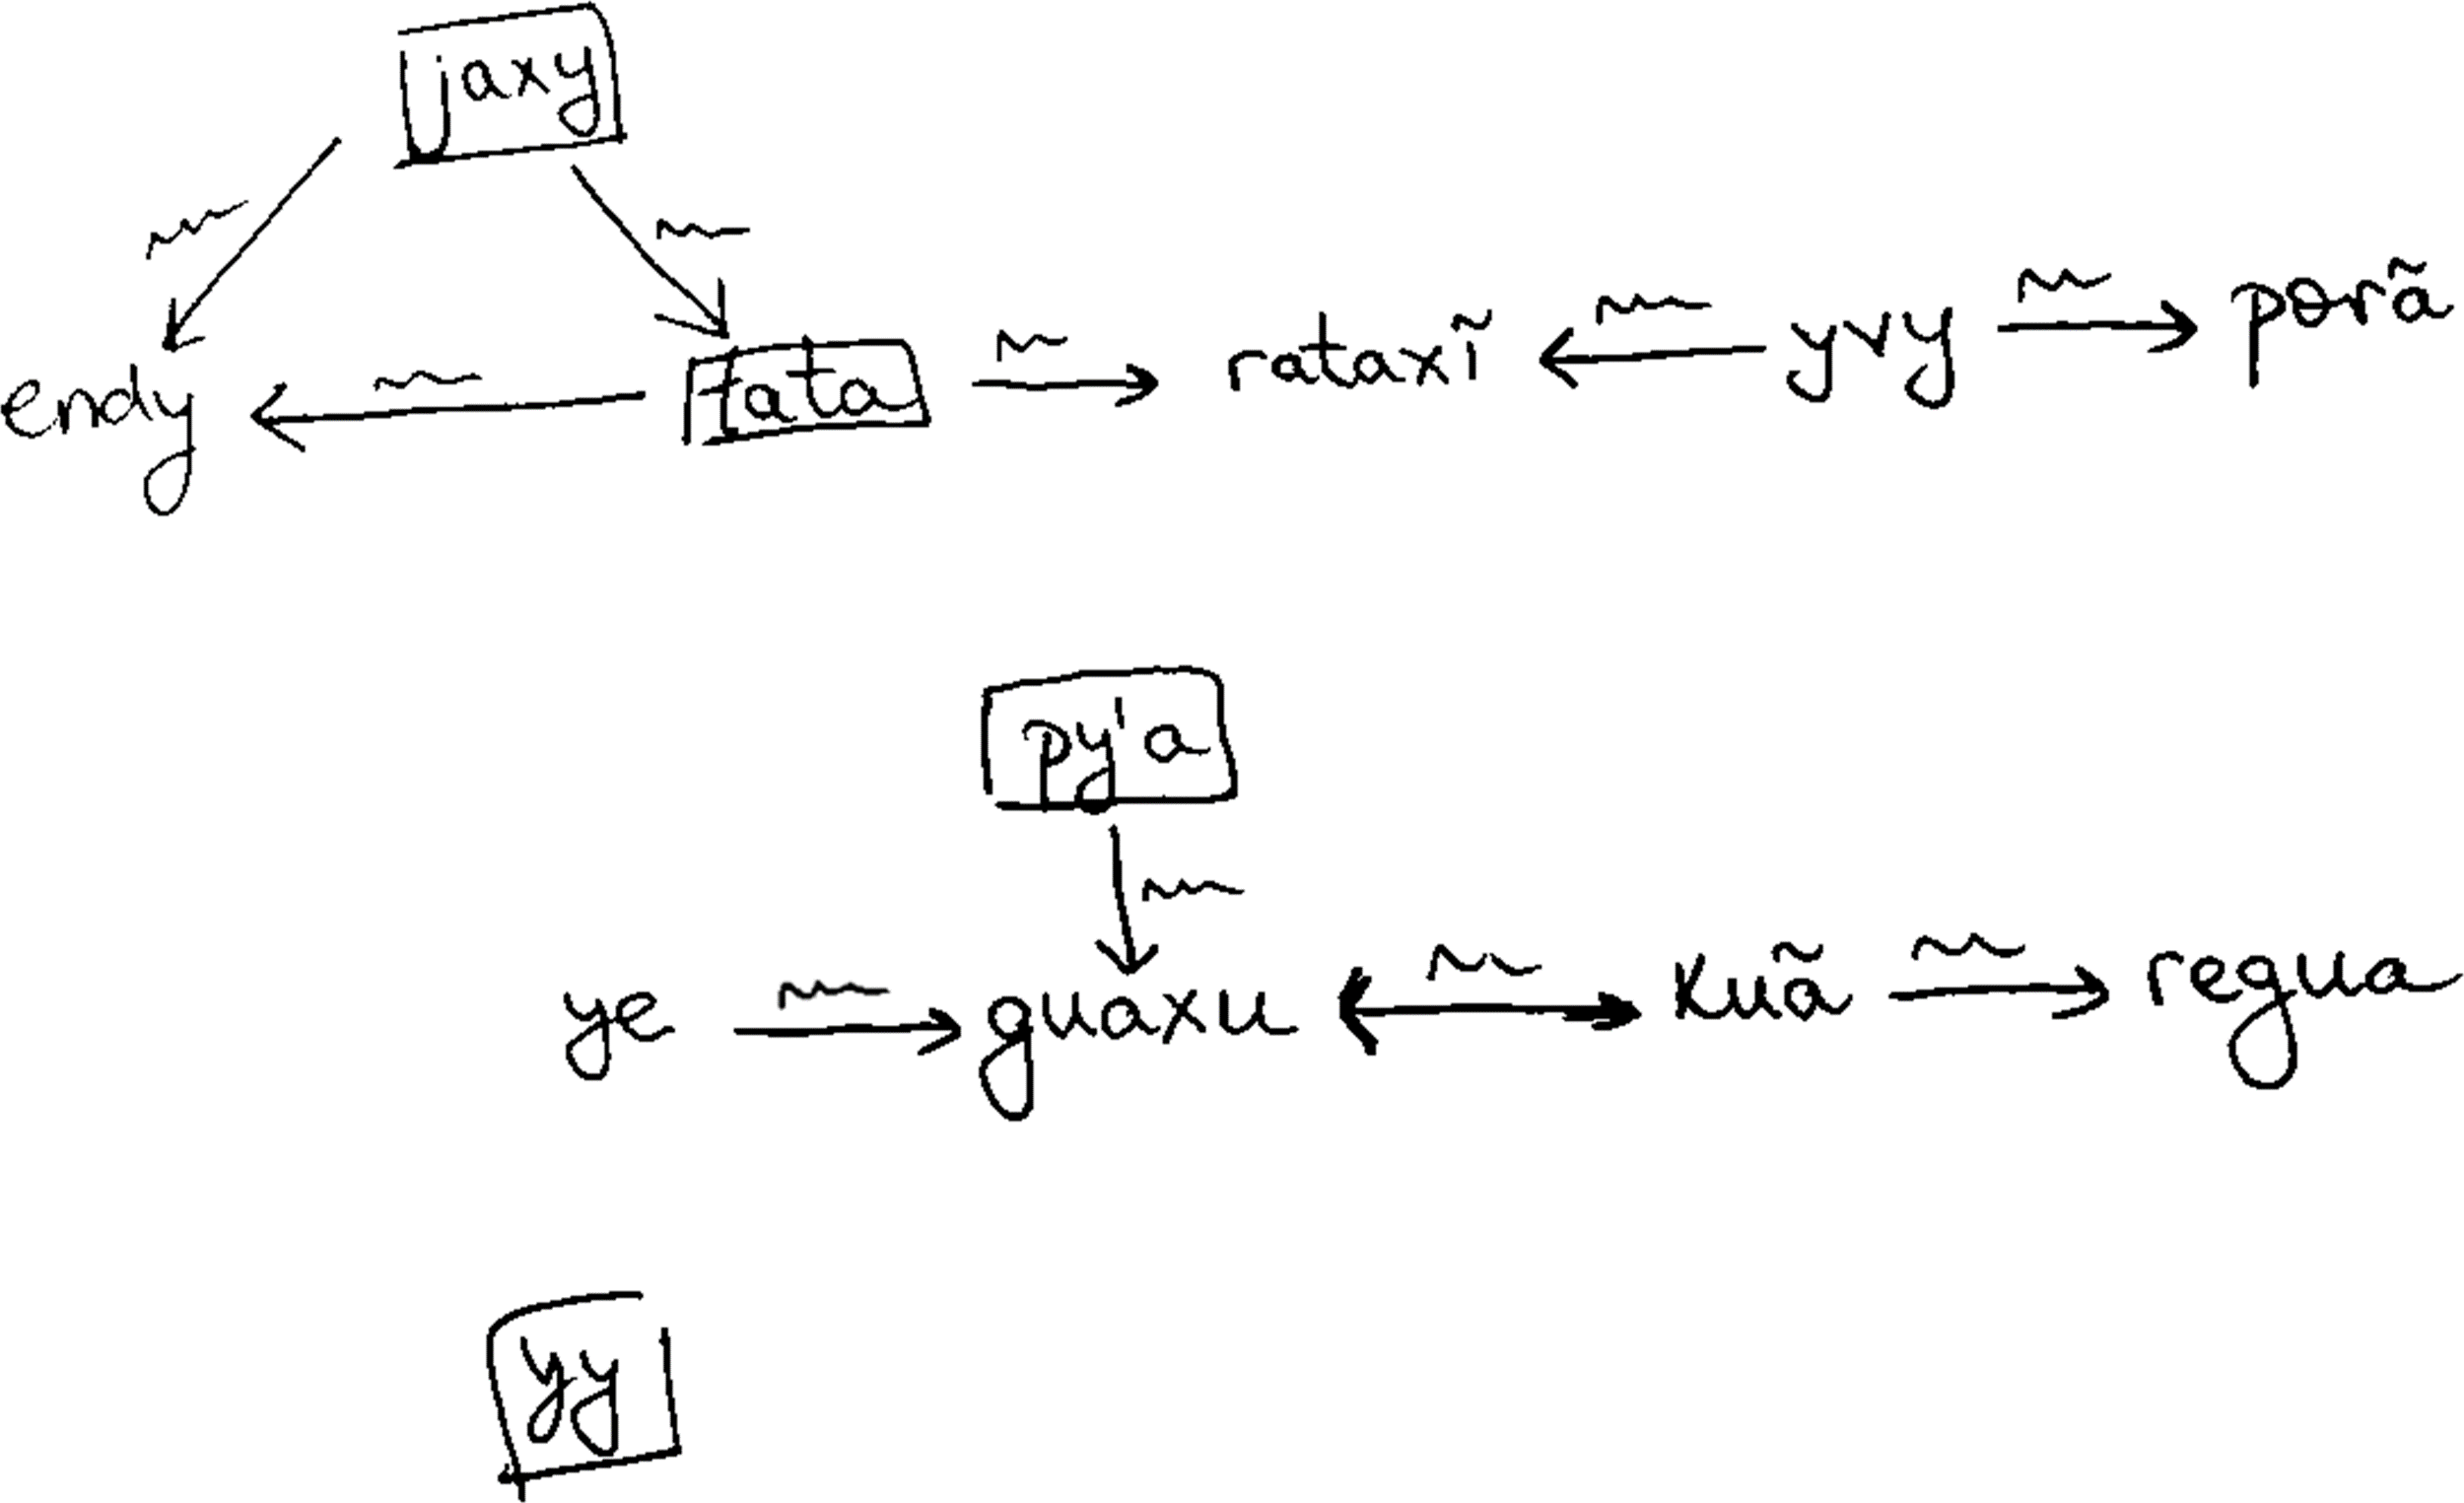
\includegraphics[width=\linewidth]{images/Handdrawn-graph-8.2.png}
\end{figure}
